% create the angle used to reduce SO2 symmetry of two states which
% are related by reflection
% use package tikz
% By Xiong
% 
% use the following command to generate the pdf
% pdflatex --jobname=sliceAngle-f1 sliceAngle.tex 

\documentclass{article}
\usepackage{graphicx}
\usepackage{tikz}

\pgfrealjobname{jacobian}

\begin{document}

\beginpgfgraphicnamed{sliceAngle-f1}
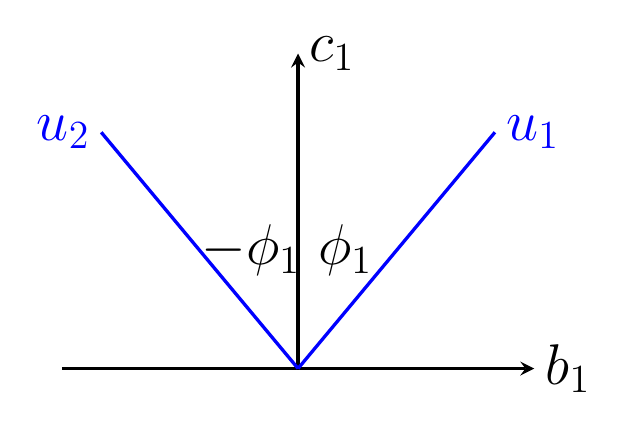
\begin{tikzpicture}

  % coordinates for the rectangle
  \coordinate (O) at (0, 0);
  \coordinate (A) at (-3, 0);
  \coordinate (B) at (3, 0);
  \coordinate (C) at (0, 4);
  \coordinate (D) at (-2.5, 3);
  \coordinate (E) at (2.5, 3);

  % draw the x - y plane
  \draw[->, >=stealth, color=black, very thick] (A) -- (B) 
  node[right=0.2]{\huge $b_1$};
  \draw[->, >=stealth, color=black, very thick] (O) -- (C) 
  node[right=0.2]{\huge $c_1$};
  
  %draw two angles
  \draw[color=blue, very thick] (O) -- (D)
  node[left=0.2]{\huge $u_2$};
  \draw[color=blue, very thick] (O) -- (E)
  node[right=0.2]{\huge $u_1$};

  \node at (0.6, 1.5) {\huge $\phi_1$} ;
  \node at (-0.6, 1.5) {\huge $-\phi_1$} ;

\end{tikzpicture}
\endpgfgraphicnamed

\end{document}